\documentclass[letter,12pt]{article}
\usepackage{graphicx}
%\usepackage{subfigure}
\usepackage{color}
\usepackage[empty,cm]{fullpage}

%\addtolength{\textwidth}{5cm}
%\addtolength{\hoffset}{-2.5cm}
%\addtolength{\textheight}{3.0cm}
%\addtolength{\voffset}{-1.5cm}


%\usepackage{geometry} % see geometry.pdf on how to lay out the page. There's lots.
%\geometry{letterpaper} % or letter or a5paper or ... etc
% \geometry{landscape} % rotated page geometry

% See the ``Article customise'' template for come common customisations

%%% BEGIN DOCUMENT
\begin{document}

\begin{center}
\textbf{FULL DAQ REBOOT CHEAT SHEET} \\

\textit{current as of March 25, 2016}
\end{center}

\begin{enumerate}

\item 
\begin{minipage}[t]{0.35\textwidth}
From the main HPS\_EPICS screen, click \texttt{DAQ Status} to open the status/reboot window.
\end{minipage}
\hspace*{0.0\textwidth}
\begin{minipage}[t]{0.55\textwidth}
\raisebox{\dimexpr-1.0\height+10pt}{ 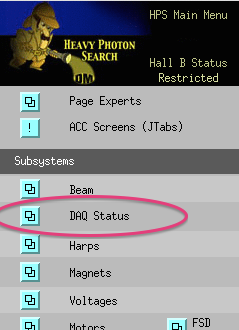
\includegraphics[width=1in]{FIX_DAQ_figures/Hps_epics_top.png}}
\end{minipage}

\item 
\begin{minipage}[t]{0.35\textwidth}
From the DAQ status/reboot window, click \texttt{Reboot FULL DAQ} and confirm the popup that appears.
\end{minipage}
\hspace*{0.0\textwidth}
\begin{minipage}[t]{0.15\textwidth}
\raisebox{\dimexpr-1.0\height+10pt}{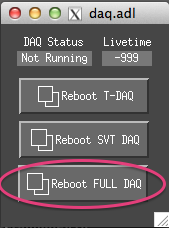
\includegraphics[width=\textwidth]{FIX_DAQ_figures/Hps_epics_fulldaqreboot.png}}
\end{minipage}
\begin{minipage}[t]{0.15\textwidth}
\raisebox{\dimexpr-1.0\height+10pt}{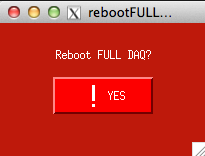
\includegraphics[width=\textwidth]{FIX_DAQ_figures/Hps_epics_fulldaqreboot_confirm.png}}
\end{minipage}

\item 
\begin{minipage}[t]{0.35\textwidth}
A terminal window will open, which may ask for the password for \texttt{clasrun}.  If so, enter it and press return. 
\end{minipage}
\hspace*{0.0\textwidth}
\begin{minipage}[t]{0.55\textwidth}
\raisebox{\dimexpr-1.0\height+10pt}{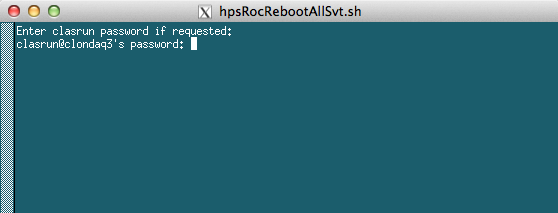
\includegraphics[width=\textwidth]{FIX_DAQ_figures/Hps_daq_reboot_1.png}}
\end{minipage}

\item 
\begin{minipage}[t]{0.35\textwidth}
After the TDAQ is rebooted, press enter to proceed to rebooting the SVT DAQ, which may again require a password.
\end{minipage}
\hspace*{0.0\textwidth}
\begin{minipage}[t]{0.55\textwidth}
\raisebox{\dimexpr-1.0\height+10pt}{
\includegraphics[width=\textwidth]{FIX_DAQ_figures/Hps_epics_svtdaqreboot_confirm.png}}
\end{minipage}

\item 
\begin{minipage}[t]{0.35\textwidth}
If the SVT DAQ reboot hangs at any point for more than a few seconds, abort with \texttt{ctrl-C} as instructed and then click the \texttt{Reboot SVT DAQ} button.
\end{minipage}
%\hspace*{0.0\textwidth}
\begin{minipage}[t]{0.4\textwidth}
\raisebox{\dimexpr-1.0\height+10pt}{
\includegraphics[width=\textwidth]{FIX_DAQ_figures/Hps_epics_svtdaqreboot_hang.png}}
\end{minipage}
\begin{minipage}[t]{0.15\textwidth}
\raisebox{\dimexpr-1.0\height+10pt}{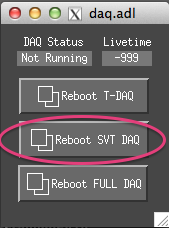
\includegraphics[width=\textwidth]{FIX_DAQ_figures/Hps_epics_svtdaqreboot.png}}
\end{minipage}
%=======================

\item After the DAQ is rebooted, check that the \textbf{FEB Status}, \textbf{IOC Status}, and \textbf{Hybrid Status} lights are all green in the SVT Summary GUI and restart the Run Control GUI: as \textbf{clasrun} on \textbf{clondaq3}, run the command... \\ 
\texttt{> runcontrol -rocs} \\
\textit{(a window on clondaq3 is probably already open with this command in history.)}\\
\end{enumerate}

This procedure should take less than ten minutes. If this procedure fails, \textbf{call the DAQ expert!!!!}

\end{document}
